\documentclass[final,twoside,article,10pt]{scrartcl}
%
\usepackage{npac}
\usepackage{amsmath}
\usepackage{url}
\usepackage{graphicx}
\usepackage[utf8]{inputenc}
\usepackage[T1]{fontenc} 
\usepackage[french]{babel}
\usepackage[fixlanguage]{babelbib}
\selectbiblanguage{french}

%
\begin{document}
%
\title{Compte Rendu de Projet de recherche de L3}
\subtitle{N\degre 4 : Problèmes \& Premiers résultats}
\author{Florian \textsc{Reynier} \& Mathis \textsc{Caristan}}
%
\date{16/02/2016}

\maketitle

\section*{Résumé de la réunion}
    Plusieurs points importants ont été abordés pendant cette réunion.
    Tout d'abord, nous avons présenté les problèmes que nous avons eu avec nos codes, en particulier avec les fonctions \textit{xxHash} et \textit{myHash}.
    Puis nous avons discuté des premiers résultats que nous avons pu obtenir avec la fonction \textit{mumrurHash}.
    Enfin, nous avons redéfini les objectifs pour les semaines à venir.

\section{Problèmes}
    Pendant les dernières semaines, nous avons fini d'écrire les codes en C pour les fonctions \textit{xxHash},\textit{myHash} et \textit{murmurHash}. Ces codes ont été compilés et executés avec succès dans des programmes entièrement écris en C. Cependant, lorsque nous avons tenté d'interfacer les codes avec OCaml, des problèmes sont apparus pour \textit{xxHash} et \textit{myHash}.
    \subsection{myHash}
        Le premier problème auquel nous avons été confronté concerne le code de \textit{myHash}.
        Comme il a été souligné plus haut, le code compile et fonctionne correctement dans un programme (de test) entièrement écrit en C, le problème provient donc de l'interface avec OCaml.
        Nous sommes pour l'instant confronté à une erreur lors de l'étape de \emph{linkage}. Nous n'avons pas encore été en mesure de comprendre la source de l'erreur. Plus de détails concernant ce problème peuvent être trouvés dans le rapport de bug \cite{bug}.
    \subsection{xxHash}
        Le second problème concerne la fonction \textit{xxHash}.
        Ici, le code compile correctement. De même, nous avons pu éxécuter le programme avec succès sur des "textes-test" d'une dizaine de clef. Le problème survient cependant sur des textes plus longs, d'environ 1000 clefs. Dans ce cas, nous obtenons systématiquement une \textbf{erreur de segmentation} provenenant de la partie C du code.
        Un travail de debogage est en cours, mais n'a pas encore porté ses fruits.

\section{Résultats}
Outre ces problèmes, nous avons été en mesure de faire fonctionner la fonction \textit{murmurHash}, et d'obtenir des résultats préliminaires.
    Afin de présenter les résultats sous forme de graphiques, nous avons choisi d'utiliser une petite table de hachage ($2^8$ valeurs de hachage), mais ce ne sera pas le cas pour l'analyse complète que nous réaliserons plus tard dans le projet.
    Les résultats sont présentés dans la figure \ref{fig:distrib}, qui présente le nombre de collisions pour chaque valeurs de hachage, et la figure \ref{fig:freq}, qui donne la fréquence de chaque nombre de collisions.
    \begin{figure}[h!]
        \begin{center}
            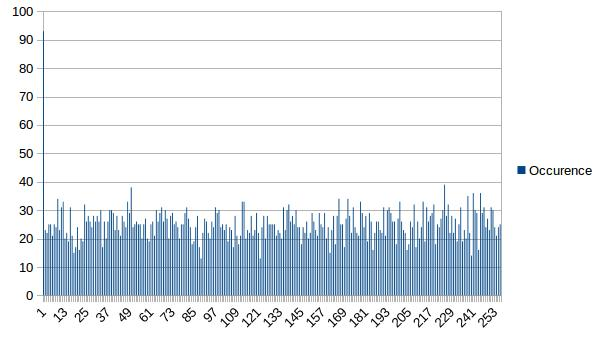
\includegraphics[width=0.65\textwidth]{./figures/hashDistribution}
            \caption{Nombre de collisions pour chaque valeur de hachage. On note la présence d'un pic au niveau de la valeur 0.}
            \label{fig:distrib}
        \end{center}
    \end{figure}
    \begin{figure}[h!]
        \begin{center}
            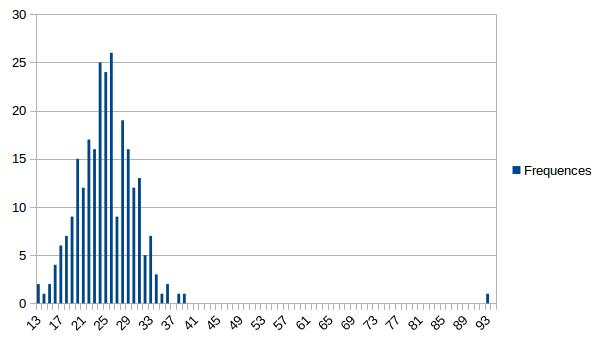
\includegraphics[width=0.65\textwidth]{./figures/frequencies}
            \caption{Frequence d'apparition d'un nombre de collisions donné. La distribution semble être gaussienne.}
            \label{fig:freq}
        \end{center}
    \end{figure}
    On note dans la première figure un pic important pour la valeur 0 (qu'on retrouve dans la seconde figure pour la valeur 93). Autrement, la distribution semble relativement homogène. Il est cependant dur de juger la distribution, avec une statistique faible (environ 6500 clefs uniques) et aucun point de comparaison. En ce qui concerne la seconde figure, il semblerait que la distribution soit Gaussienne, bien qu'encore une fois, il soit dur de juger pour les mêmes raisons que précédemment.

\section*{Objectifs}
    L'objectif a court terme est tout d'abord de résoudre les problèmes que nous avons rencontré avec les fonctions \textit{xxHash} et \textit{myHash} afin de pouvoir obtenir des résultats comparables à ceux obtenus avec \textit{murmurHash}.
    Dans un second temps, nous comptons augmenter la statistique afin de pouvoir mieux caractériser nos résultats.
    Sur ce point, plusieurs idées ont été envisagées.
    La plus simple consiste simplement à considérer la suite du texte que nous avons utilisé pour le moment. Une autre consiste à réutiliser le même texte, mais après lui avoir fait subir un chiffrement de César. Enfin, une dernière idée est de toujours garder le même texte, mais de considérer 8 bits de la valeur de hachage différents (actuellement, nous utilisons les 8 premiers, sur 32).
    Un dernier point de moindre importance qui a été soulevé, est de remplacer quand c'est possible les divisions entières par des décallages de bits (opérateur \textbf{>{}>} en C).

\begin{thebibliography}{9}
    \bibitem{bug}
        Florian Reynier, Mathis Caristan, \emph{Rapport de bug \textit{myHash} 1}.
\end{thebibliography}




\end{document}
